\documentclass[]{article}
\newcommand{\FileDepth}{../../..}
\usepackage[letterpaper, landscape, margin=0.5cm]{geometry}
\usepackage[T1]{fontenc}
\usepackage{textcomp}%Not strictly necessary, but gives \textmu command for "micro."
\usepackage{fancyhdr}
\usepackage{amsmath}
\usepackage{amssymb}
\usepackage{graphicx}
\usepackage{xcolor}
\usepackage{tikz}
\usetikzlibrary{calc}
\usepackage[shortlabels]{enumitem}
\usepackage{multicol}
\usepackage{vwcol}
\usepackage{hyperref}
\usepackage{wrapfig}
%opening
\newcommand{\SecType}{S}
\newcommand{\Week}{3}
\title{PH 211 Studio \Week}
\author{Benjamin Bauml}
\date{Summer 2024}

\newcommand{\Purpose}{4}
\newcommand{\DefOnly}{0}

\input{\FileDepth/Formats/Assignment20240614.tex}
\usepackage[absolute]{textpos}
% This package relies on Assignment Format 2024-06-14 or later to work. It is recommended that the Purpose and DefOnly commands be given as such:
%\newcommand{\Purpose}{4}
%\newcommand{\DefOnly}{0}
% Activities need to be entered outside of the TeacherMargin and PresentSpace environments, otherwise they will be defined only locally. They can even go in the preamble.
\newenvironment{TeacherMargin}{\begin{textblock*}{10.8cm}(0.5cm,0.5cm)
\small}{\end{textblock*}
\hspace{0.1cm}}
\newenvironment{PresentSpace}{\begin{textblock*}{0.3cm}(26.85cm,9.35cm)
--
\end{textblock*}
\begin{textblock*}{15.6cm}(11.8cm,0.5cm)
\begin{Repurpose}{1}
\Large}{\end{Repurpose}
\end{textblock*}
\hspace{0.1cm}}

%\newcommand{\FBDaxes}[4][2]{
	\begin{scope}[shift={(#2)},rotate=#3]
		% x-axis
		\draw[thick,->] (-#1,0) -- (#1,0);
		\node[anchor=west] at (#1,0) {$x$};
		% y-axis
		\draw[thick,->] (0,-#1) -- (0,#1);
		\node[anchor=south] at (0,#1) {$y$};
		\coordinate (#4) at (0,0);
	\end{scope}
}
\newcommand{\FBDvectorMA}[4]{
	\begin{scope}[shift={(#1)}]
		\coordinate (#4tip) at ({#2*cos(#3)},{#2*sin(#3)});
		\draw[ultra thick,blue,->] (#1) -- (#4tip);
	\end{scope}
}
\newcommand{\FBDvectorXY}[3]{
	\begin{scope}[shift={(#1)}]
		\coordinate (#3tip) at (#2);
		\draw[ultra thick,blue,->] (0,0) -- (#3tip);
	\end{scope}
}
\newcommand{\FBDdot}[1]{
	\filldraw[black] (#1) circle (3pt);
}
\newcommand{\FBDbox}[5][1]{
	\begin{scope}[shift={(#2)},rotate=#3]
		\filldraw[color=black,fill=white,thick] ({-#1/2},{#1/2}) -- ({-#1/2},{-#1/2}) -- ({#1/2},{-#1/2}) -- ({#1/2},{#1/2}) -- cycle;
		% Left side coordinates
		\coordinate (#4ltq) at ({-#1/2},{#1/4});
		\coordinate (#4lcent) at ({-#1/2},0);
		\coordinate (#4lbq) at ({-#1/2},{-#1/4});
		% right side coordinates
		\coordinate (#4rtq) at ({#1/2},{#1/4});
		\coordinate (#4rcent) at ({#1/2},0);
		\coordinate (#4rbq) at ({#1/2},{-#1/4});
		% top coordinates
		\coordinate (#4tlq) at ({-#1/4},{#1/2});
		\coordinate (#4tcent) at (0,{#1/2});
		\coordinate (#4trq) at ({#1/4},{#1/2});
		% bottom coordinates
		\coordinate (#4blq) at ({-#1/4},{-#1/2});
		\coordinate (#4bcent) at (0,{-#1/2});
		\coordinate (#4brq) at ({#1/4},{-#1/2});
		% corners
		\coordinate (#4tl) at ({-#1/2},{#1/2});
		\coordinate (#4tr) at ({#1/2},{#1/2});
		\coordinate (#4bl) at ({-#1/2},{-#1/2});
		\coordinate (#4br) at ({#1/2},{-#1/2});
		\node at (0,0) {#5};
	\end{scope}
}
%\newcommand{\MVec}[3][0]{%Creates a momentum vector of length #3 centered at #2 and rotated #1 degrees counterclockwise.
	\begin{scope}[rotate=#1,shift={(#2)}]
		\draw[->,thick] ({-#3/2},0) -- ({#3/2},0);
	\end{scope}
}
\newcommand{\MDot}[1]{%Creates a dot at #1 to represent a zero vector.
	\filldraw (#1) circle (1pt);
}
\newcommand{\MVDRows}[2][4.5]{%Creates the rows (initial, delta, final) of a momentum vector diagram. The optional argument determines the width of the table, and defaults to a good length for three columns (two objects and the total system). The non-optional argument gives a coordinate name (not displayed) to the diagram.
	\begin{scope}
		%\draw[thick] (0,5.5) -- (0,0);
		\draw[thick] (-1,4.5) -- (#1,4.5);
		\node at (-0.5,3.75) {$\vec{p}_{i}$};
		\draw[thick] (-1,3) -- (#1,3);
		\node at (-0.5,2.25) {$\Delta\vec{p}$};
		\draw[thick] (-1,1.5) -- (#1,1.5);
		\node at (-0.5,0.75) {$\vec{p}_{f}$};
		\coordinate (#2) at (0,5);
	\end{scope}
}
\newcommand{\MVDCol}[4][0.75]{%Creates a column for an object in a momentum vector diagram. The first (non-optional) argument is the coordinate name (not displayed) of the column, while the second is the displayed column header. The first argument also names the three entries down the column. The third argument anchors the column, so it should either be the coordinate name of the MVD (for the first column) or the coordinate name of the previous column. The optional argument indicates how far the center of the column should be from the previous column's edge, and defaults to 0.75.
	\begin{scope}[shift={(#4)}]
		\node at (#1,0) {#3};
		%\draw[thick] ({#1*2},0.5) -- ({#1*2},-5);
		\draw[thick] (0,0.5) -- (0,-5);
		\coordinate (#2init) at (#1,-1.25);
		\coordinate (#2delt) at (#1,-2.75);
		\coordinate (#2fin) at (#1,-4.25);
		\coordinate (#2) at ({#1*2},0);
	\end{scope}
}

%\input{\FileDepth/Activities/Activity_One/Activity_One.tex}
%\input{\FileDepth/Activities/Activity_Two/Activity_Two.tex}

\begin{document}
\begin{TeacherMargin}

\end{TeacherMargin}
\begin{PresentSpace}
\begin{center}
	\huge Studio 3: Motion and Forces \\
	\vspace{1cm}
	\LARGE Choose your own seats today (still at tables 2, 3, 6, 7).
\end{center}
%\underline{Warm-Up Activity} \\
%How is acceleration symbolically related to velocity? WRITE BIG!
\begin{comment}{2}
\begin{enumerate}[(A)]
	\item Velocity is acceleration times $t$.
	\vspace{6pt}
	\item Acceleration is velocity times $t$.
	\vspace{15pt}
	\item Acceleration is the derivative of velocity.
	\item Velocity is the derivative of acceleration.
\end{enumerate}
\end{comment}
\end{PresentSpace}
\newpage
\begin{TeacherMargin}
	\noindent\textbf{From the Syllabus}
	
	Projects are assignments where you will demonstrate and synthesize what you have learned over many weeks. Projects may take many different potential forms, including written, visual, or video. Almost every week (except for weeks with ungrading), there will be some milestone to complete in this project, such as setting group expectations (if you work in a group), proposing a project, submitting a rough draft, peer reviewing other classmates’ projects, and submitting a final draft. All project milestones are due on Fridays.
	
	The standard format for projects that you can expect if you continue on to 212 is a group assignment (usually 3 students), consisting of a 10-15 minute video solution to a physics problem, with a full calculation, sensemaking, and reflection. You may choose to get used to this format in preparation for continuing on in the sequence, or you can take this opportunity to be more creative in how you approach the project. I vehemently encourage you to find some idea for a project that excites you, be it creating an educational video or report, performing research, melding physics with something artistic, or even something I haven’t considered as a possible physics project yet.
	
	\noindent\textbf{From the Group Expectations Assignment}
	
	To complete this in-class assignment, you must come up with an agreement together with your group on how you plan to work on the project together. Fill out the questions provided based on group discussion. \textit{Only one group member needs to fill this out.}
	
	There are many different ways to plan together. It is your job as a group to negotiate how each member will contribute to the project, with regards to participation, communication, meeting together, individual conduct, handling conflict, and completing the project.
	
	As you answer the prompts provided, think back on what has made your past group experiences positive, dreary, rewarding, frustrating, satisfying, stressful, etc. What qualities would you like to ideally have in how your group approaches this group project?
\end{TeacherMargin}
\begin{PresentSpace}
	\textbf{Project Information}
	\begin{itemize}
		\item Demonstrate and synthesize what you have learned over many weeks.
		\item Many possible forms, such as written, visual, or video.
		\item Milestones due Fridays at 8pm (almost) every week:
		\begin{itemize}
			\item Setting group expectations (Week 2)
			\begin{itemize}
				\item Once you have your group, you will work with them in lecture and studio.
			\end{itemize}
			\item Project proposal (Week 3)
			\item Rough draft (Week 5)
			\item Peer review (Week 6)
			\item Final draft (Week 7)
		\end{itemize}
	\end{itemize}
	\textbf{What to Expect in PH 212}
	\begin{itemize}
		\item 10-15 minute video presentation by group (usually 3 students)
		\item Solution to a physics problem, or presentation on self-taught topic (such as buoyant force or drag force)
		\item Calculation, sensemaking, and reflection
	\end{itemize}
	\textbf{Your Options}
	\begin{itemize}
		\item 212 format (get used to it for 212)
		\item Some other idea that excites you!
		\begin{itemize}
			\item Educational video or report
			\item Research
			\item Melding physics with something artistic
			\item Surprise me!
		\end{itemize}
		\item If it doesn't involve enough calculation, sensemaking, and reflection, I may request modifications.
	\end{itemize}
\end{PresentSpace}
\newpage
\begin{TeacherMargin}

\end{TeacherMargin}
\begin{PresentSpace}
\textbf{Project Brainstorm}
\begin{itemize}
	\item With your neighbors, come up with as many creative ideas for projects as you can.
	\begin{itemize}
		\item A proposed problem should relate to motion and things that affect motion.
		\item Basic formats include written work and videos. Can you suggest an interesting subcategory of either of those formats, or perhaps a new format entirely?
	\end{itemize}
	\item I will write as many ideas of yours as I can on this slide, along with the names of the people who came up with them.
\end{itemize}
\end{PresentSpace}
\newpage
\begin{TeacherMargin}
Let us choose a standard coordinate system, with $\hat{y}$ pointing toward the top of the page, and $\hat{x}$ pointing to the right. We are allowed to place the origin at $t_{0}$, which I will do for simplicity and consistency. A small {\color{red}red} set of axes will mark the origin.

My velocity vectors will be in {\color{blue}blue}, and my acceleration vectors in {\color{purple}purple}. The arrows only need to be qualitatively accurate for this activity, but the ones I did below are quantitatively accurate up to overall scaling.
\begin{center}
	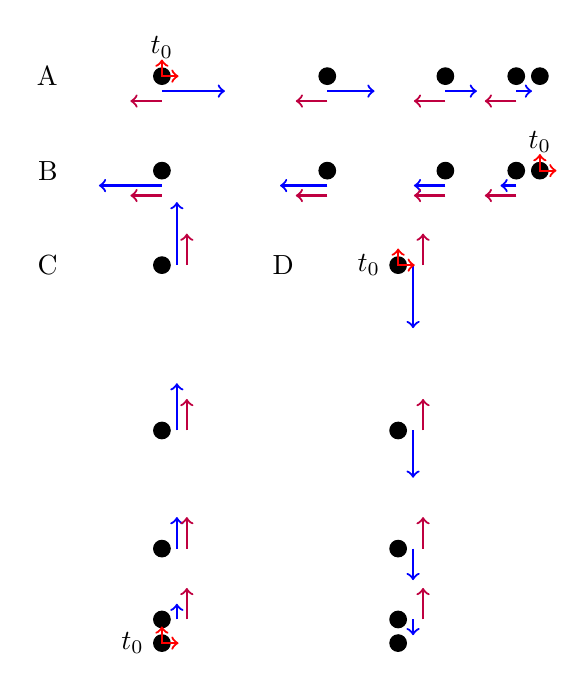
\begin{tikzpicture}
		\begin{scope}[scale=0.6,shift={(0,0)}]
			\foreach \t in {0,1,2,3,4}
				\filldraw ({4*\t-\t*\t/2},0) circle (5pt);
			\foreach \t in {0,1,2,3}
				\draw[thick,->,blue] ({4*\t-\t*\t/2},{-9pt}) -- ({4*\t-\t*\t/2+(4-\t)/3},{-9pt});
			\foreach \t in {0,1,2,3}
				\draw[thick,->,purple] ({4*\t-\t*\t/2},{-15pt}) -- ({4*\t-\t*\t/2-2/3},{-15pt});
			\node[anchor=south] at (0,5pt) {$t_{0}$};
			\node[anchor=east] at (-2,0) {A};
			\begin{scope}[shift={(0,0)}]
				\draw[red,thick,<->] (0,10pt) -- (0,0) -- (10pt,0);
			\end{scope}
		\end{scope}
		\begin{scope}[scale=0.6,shift={(0,-2)}]
			\foreach \t in {0,1,2,3,4}
				\filldraw ({4*\t-\t*\t/2},0) circle (5pt);
			\foreach \t in {0,1,2,3}
				\draw[thick,->,blue] ({4*\t-\t*\t/2},{-9pt}) -- ({4*\t-\t*\t/2-(4-\t)/3},{-9pt});
			\foreach \t in {0,1,2,3}
				\draw[thick,->,purple] ({4*\t-\t*\t/2},{-15pt}) -- ({4*\t-\t*\t/2-2/3},{-15pt});
			\node[anchor=south] at (8,5pt) {$t_{0}$};
			\node[anchor=east] at (-2,0) {B};
			\begin{scope}[shift={(8,0)}]
				\draw[red,thick,<->] (0,10pt) -- (0,0) -- (10pt,0);
			\end{scope}
		\end{scope}
		%\begin{scope}[scale=0.6,shift={(13,0)}]
		\begin{scope}[scale=0.6,shift={(0,-4)}]
			\foreach \t in {0,1,2,3,4}
				\filldraw (0,{-4*\t+\t*\t/2}) circle (5pt);
			\foreach \t in {0,1,2,3}
				\draw[thick,->,blue] ({9pt},{-4*\t+\t*\t/2}) -- ({9pt},{-4*\t+\t*\t/2+(4-\t)/3});
			\foreach \t in {0,1,2,3}
				\draw[thick,->,purple] ({15pt},{-4*\t+\t*\t/2}) -- ({15pt},{-4*\t+\t*\t/2+2/3});
			\node[anchor=east] at (-5pt,-8) {$t_{0}$};
			\node[anchor=east] at (-2,0) {C};
			\begin{scope}[shift={(0,-8)}]
				\draw[red,thick,<->] (0,10pt) -- (0,0) -- (10pt,0);
			\end{scope}
		\end{scope}
		%\begin{scope}[scale=0.6,shift={(18,0)}]
		\begin{scope}[scale=0.6,shift={(5,-4)}]
			\foreach \t in {0,1,2,3,4}
				\filldraw (0,{-4*\t+\t*\t/2}) circle (5pt);
			\foreach \t in {0,1,2,3}
				\draw[thick,->,blue] ({9pt},{-4*\t+\t*\t/2}) -- ({9pt},{-4*\t+\t*\t/2-(4-\t)/3});
			\foreach \t in {0,1,2,3}
				\draw[thick,->,purple] ({15pt},{-4*\t+\t*\t/2}) -- ({15pt},{-4*\t+\t*\t/2+2/3});
			\node[anchor=east] at (-5pt,0) {$t_{0}$};
			\node[anchor=east] at (-2,0) {D};
			\begin{scope}[shift={(0,0)}]
				\draw[red,thick,<->] (0,10pt) -- (0,0) -- (10pt,0);
			\end{scope}
		\end{scope}
	\end{tikzpicture}
\end{center}
\begin{enumerate}[(A)]
	\item Acceleration is negative, velocity is positive.
	\begin{itemize}
		\item The object is slowing down.
	\end{itemize}
	\item Acceleration is negative, velocity is negative.
	\begin{itemize}
		\item The object is speeding up.
	\end{itemize}
	\item Acceleration is positive, velocity is positive.
	\begin{itemize}
		\item The object is speeding up.
	\end{itemize}
	\item Acceleration is positive, velocity is negative.
	\begin{itemize}
		\item The object is slowing down.
	\end{itemize}
\end{enumerate}
An object gains speed when $\vec{v}$ and $\vec{a}$ point in the same direction (both positive or both negative in 1-D), and it gets slower when $\vec{v}$ and $\vec{a}$ are in opposite directions. ``Negative acceleration'' does NOT mean slowing down!

\noindent\textbf{Position} \\
Above, the given origins make position positive (or zero) for all points in A and C, and negative (or zero) for all points in B and D. Position is the only vector of the given three that depends on the origin. Moving the origin doesn't affect how the directions of velocity and acceleration are aligned with the axes.

If, for example, I shifted the origin in D to the right, then the position vectors in D wouldn't have a well-defined sign at all. We can use sign to indicate direction only when a vector is aligned with a coordinate axis.
\end{TeacherMargin}
\begin{PresentSpace}
\vspace{-10pt}
\section*{S2-1: Strobes and Origins}
\vspace{-10pt}
The initial position in each strobe diagram is labeled $t_{0}$. For each case:
\begin{multicols}{2}
\begin{itemize}
	\item Choose a coordinate system (use the same system for all cases).
	\vspace{10pt}
	\item Sketch velocity vectors for each point.
	\item Sketch acceleration vectors for each point.
	\item Identify whether each of the following is positive or negative:
	\begin{itemize}
		\item Position
		\item Velocity
		\item Acceleration
	\end{itemize}
\end{itemize}
%\end{multicols}
\begin{center}
	\begin{tikzpicture}
		\begin{scope}[scale=0.6,shift={(0,0)}]
			\foreach \t in {0,1,2,3,4}
				\filldraw ({4*\t-\t*\t/2},0) circle (5pt);
			\node[anchor=south] at (0,5pt) {$t_{0}$};
			\node[anchor=east] at (-2,0) {A};
		\end{scope}
		\begin{scope}[scale=0.6,shift={(0,-2)}]
			\foreach \t in {0,1,2,3,4}
				\filldraw ({4*\t-\t*\t/2},0) circle (5pt);
			\node[anchor=south] at (8,5pt) {$t_{0}$};
			\node[anchor=east] at (-2,0) {B};
		\end{scope}
		%\begin{scope}[scale=0.6,shift={(13,0)}]
		\begin{scope}[scale=0.6,shift={(0,-4)}]
			\foreach \t in {0,1,2,3,4}
				\filldraw (0,{-4*\t+\t*\t/2}) circle (5pt);
			\node[anchor=east] at (-5pt,-8) {$t_{0}$};
			\node[anchor=east] at (-2,0) {C};
		\end{scope}
		%\begin{scope}[scale=0.6,shift={(18,0)}]
		\begin{scope}[scale=0.6,shift={(5,-4)}]
			\foreach \t in {0,1,2,3,4}
				\filldraw (0,{-4*\t+\t*\t/2}) circle (5pt);
			\node[anchor=east] at (-5pt,0) {$t_{0}$};
			\node[anchor=east] at (-2,0) {D};
		\end{scope}
	\end{tikzpicture}
\end{center}
\end{multicols}
\end{PresentSpace}
\newpage
\begin{TeacherMargin}
\begin{comment}
	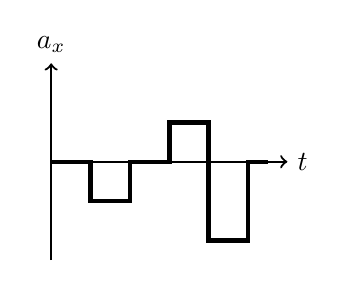
\begin{tikzpicture}[scale=0.5]
		\draw[thick,->] (0,-2.5) -- (0,2.5) node[anchor=south] {$a_{x}$};
		\draw[thick,->] (0,0) -- (6,0) node[anchor=west] {$t$};
		\draw[ultra thick] (0,0) -- (1,0) -- (1,-1) -- (2,-1) -- (2,0) -- (3,0) -- (3,1) -- (4,1) -- (4,-2) -- (5,-2) -- (5,0) -- (5.5,0);
	\end{tikzpicture}
\end{comment}
From the acceleration graph, we can tell things about both the position and velocity graphs.
\begin{itemize}
	\item The velocity graph is piecewise linear. It will have corners where the acceleration graph has jump discontinuities, but everywhere the acceleration graph is constant, the velocity graph will be linear with a slope corresponding to the value of the acceleration.
	\item The acceleration is the second derivative of position, so its sign characterizes the concavity of the position graph. Where $a_{x}$ is positive, the position graph will be concave up, and where $a_{x}$ is negative, the position graph will be concave down.
\end{itemize}
The acceleration does not tell us anything about the initial speed or initial position. I will demonstrate two graphs for $v_{x}$ with two different initial speeds in two different colors. Changing the initial speed shifts the graph vertically, but does not change its shape.
\begin{center}
	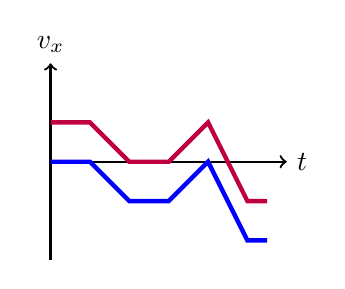
\begin{tikzpicture}[scale=0.5]
		\draw[thick,->] (0,-2.5) -- (0,2.5) node[anchor=south] {$v_{x}$};
		\draw[thick,->] (0,0) -- (6,0) node[anchor=west] {$t$};
		\draw[ultra thick,blue] (0,0) -- (1,0) -- (2,-1) -- (3,-1) -- (4,0) -- (5,-2) -- (5.5,-2);
		\draw[ultra thick,purple,shift={(0,1)}] (0,0) -- (1,0) -- (2,-1) -- (3,-1) -- (4,0) -- (5,-2) -- (5.5,-2);
	\end{tikzpicture}
\end{center}
From this graph, we can learn even more about the position graph.
\begin{itemize}
	\item The position graph is smooth, meaning its slope matches at every point and there are no corners. Since velocity is continuous, the derivative of position is well defined at every point.
	\item Where velocity is constant, the position graph is linear, and where velocity is linear and not constant, the position graph will be parabolic. When velocity is increasing, the slope of position is getting more positive (which mean getting steeper for positive slope, but flatter for negative slope), and when velocity is decreasing, the slope of position is getting more negative (which mean getting steeper for negative slope, but flatter for positive slope).
\end{itemize}
We can pick any initial position, but that just shifts the graph, so let's start it off at zero for simplicity. However, the choice of initial velocity affected the sign of the slope everywhere, so it actually has a radical effect on the graph's shape.
\begin{center}
	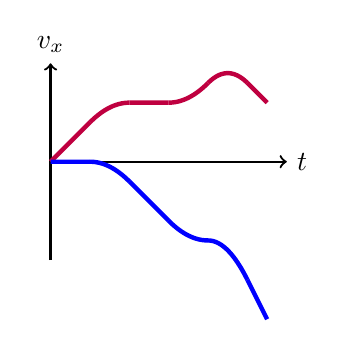
\begin{tikzpicture}[scale=0.5]
		\draw[thick,->] (0,-2.5) -- (0,2.5) node[anchor=south] {$v_{x}$};
		\draw[thick,->] (0,0) -- (6,0) node[anchor=west] {$t$};
		\draw[ultra thick,purple] (0,0) -- (1,1) (2,1.5) -- (3,1.5) (5,2) -- (5.5,1.5);
		\draw[ultra thick,purple,domain=0:1,variable=\t] plot (\t+1,{1+\t-\t*\t/2});
		\draw[ultra thick,purple,domain=0:1,variable=\t] plot (\t+3,{1.5+\t*\t/2});
		\draw[ultra thick,purple,domain=0:1,variable=\t] plot (\t+4,{2+\t-\t*\t});
		\draw[ultra thick,blue] (0,0) -- (1,0) (2,-0.5) -- (3,-1.5) (5,-3) -- (5.5,-4);
		\draw[ultra thick,blue,domain=0:1,variable=\t] plot (\t+1,{-\t*\t/2});
		\draw[ultra thick,blue,domain=0:1,variable=\t] plot (\t+3,{-1.5-\t+\t*\t/2});
		\draw[ultra thick,blue,domain=0:1,variable=\t] plot (\t+4,{-2-\t*\t});
	\end{tikzpicture}
\end{center}
\end{TeacherMargin}
\begin{PresentSpace}
\vspace{-10pt}
\section*{S2-2: Graphing Acceleration, Velocity, Position}
\vspace{-10pt}
Below is a graph of $a$ vs. $t$ for a car. Draw and label graphs of $v$ vs. $t$ and $x$ vs. $t$ for the car.
\begin{center}
	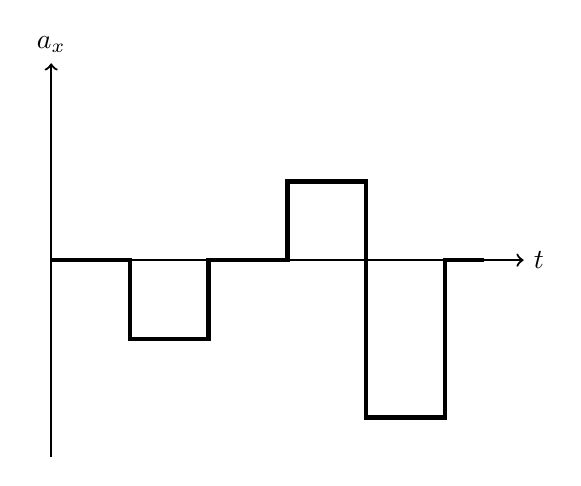
\begin{tikzpicture}
		\draw[thick,->] (0,-2.5) -- (0,2.5) node[anchor=south] {$a_{x}$};
		\draw[thick,->] (0,0) -- (6,0) node[anchor=west] {$t$};
		\draw[ultra thick] (0,0) -- (1,0) -- (1,-1) -- (2,-1) -- (2,0) -- (3,0) -- (3,1) -- (4,1) -- (4,-2) -- (5,-2) -- (5,0) -- (5.5,0);
	\end{tikzpicture}
\end{center}
\end{PresentSpace}
\newpage
\begin{TeacherMargin}

\end{TeacherMargin}
\begin{PresentSpace}
\section*{Main Ideas}
\begin{itemize}
	\item Speed increases when velocity and acceleration are in the same direction. Speed decreases when velocity and acceleration are in opposite directions.
	\item Position depends on the choice of origin.
	\item Acceleration tells you about the slope of the velocity graph and the concavity of the position graph, but it does not tell you about their initial values.
	\item Velocity tells you about the slope of the position graph. Changing the initial velocity shifts all of the values of velocity, which changes the overall shape of the position graph.
\end{itemize}
\end{PresentSpace}
\end{document}